\documentclass[lettersize,journal]{IEEEtran}
\usepackage{amsmath,amsfonts}
\usepackage{algorithmic}
\usepackage{array}
\usepackage{textcomp}
\usepackage{stfloats}
\usepackage{url}
\usepackage{verbatim}
\usepackage{graphicx}
\usepackage{algorithm}
\usepackage{array}
\usepackage{cite}
\usepackage{subfigure}
\usepackage{kotex}
\usepackage{bbm}
\usepackage{hyperref}
\usepackage{xcolor} % 삭제 예정
\newcommand{\tred}{\textcolor{red}}
\newcommand{\tblue}{\textcolor{blue}}

\hyphenation{op-tical net-works semi-conduc-tor IEEE-Xplore}
\def\BibTeX{{\rm B\kern-.05em{\sc i\kern-.025em b}\kern-.08em
    T\kern-.1667em\lower.7ex\hbox{E}\kern-.125emX}}

\newcolumntype{M}[1]{>{\centering\arraybackslash}m{#1}}
\usepackage{balance}
\begin{document}
\title{Novel Channel Estimation Method Based on Enhanced Diffusion Posterior Sampling for Massive MIMO Systems}

\author{\IEEEauthorblockN{Jinwook Kim,~\IEEEmembership{Graduate Student Member,~IEEE}},  \IEEEauthorblockN{Seongwoo Lee,~\IEEEmembership{Graduate Student Member,~IEEE}},

\IEEEauthorblockN{Joonho Seon,~\IEEEmembership{Graduate Student Member,~IEEE}}, \IEEEauthorblockN{Soo Hyun Kim,~\IEEEmembership{Member,~IEEE}}, \IEEEauthorblockN{Young Ghyu Sun,~\IEEEmembership{Member,~IEEE}},

\IEEEauthorblockN{Hyowoon Seo,~\IEEEmembership{Member,~IEEE}}, \IEEEauthorblockN{Dong In Kim,~\IEEEmembership{Life Fellow,~IEEE}}, and \IEEEauthorblockN{Jin Young Kim,~\IEEEmembership{Senior Member,~IEEE}
\vspace{-10pt}
}
        % <-this % stops a space
\thanks{This work was 
partly supported by Institute of Information \& communications Technology Planning \& Evaluation (IITP) grant funded by the Korea government (MSIT) (No. 2021-0-00892-005, Research on advanced physical layer technologies of low-earth orbit (LEO) satellite communication systems for ubiquitous intelligence in space) and 
supported by the MSIT(Ministry of Science and ICT), Korea, under the ITRC(Information Technology Research Center) support program(IITP-2025-RS-2023-00258639) supervised by the IITP(Institute for Information \& Communications Technology Planning \& Evaluation). (\it{Corresponding author: Jin Young Kim.})}% <-this % stops a space
\thanks{Jinwook Kim, Seongwoo Lee, Joonho Seon, Soo Hyun Kim, Young Ghyu Sun, and Jin Young Kim are with the Department of Electronic Convergence Engineering, Kwangwoon University, Seoul 01897, South Korea (e-mail: \{yoonlight12, swoo1467, dimlight13, kimsoogus, yakrkr, jinyoung\}@kw.ac.kr).}
\thanks{Hyowoon Seo, and Dong In Kim are with the Department of Electrical and Computer Engineering, Sungkyunkwan University, Suwon 16419, South Korea (e-mail: \{hyowoonseo, dongin\}@skku.edu).}}


% The paper headers
\markboth{IEEE communications letters, ~Vol.~15, No.~8, August~2025}%
{Shell \MakeLowercase{\textit{et al.}}: A Sample Article Using IEEEtran.cls for IEEE Journals}

\maketitle
\begin{abstract}
In this letter, a novel diffusion model (DM)-based channel estimation method is proposed to mitigate the abrupt performance degradation in massive multiple-input multiple-output (MIMO) systems under severe pilot scarcity. To address this issue, the proposed method jointly exploits first- and second-order posterior moments via the moment matching principle and Tweedie’s formula. This method improves estimation accuracy and robustness against high uncertainties, while reducing computational burden. From the simulation results, it is confirmed that the proposed method successfully mitigates the abrupt performance degradation. The proposed method also substantially outperforms state-of-the-art DM-based methods in estimation accuracy under severe pilot-scarce conditions, while achieving comparable computational complexity.
\end{abstract}

\begin{IEEEkeywords}
Channel estimation, massive MIMO, diffusion model, moment matching, Tweedie's formula.
\end{IEEEkeywords}


\section{Introduction}

Massive multiple-input-multiple-output (MIMO) systems have emerged as a key technology for future 6G communication systems~\cite{busariMillimeterWaveMassiveMIMO2018}. To fully exploit its potential, accurate acquisition of channel state information (CSI) is indispensable. However, a fundamental limitation is that the number of pilot symbols required for channel estimation scales linearly with the massive number of antennas. This limitation leads to a severe pilot overhead bottleneck which directly degrades the spectral efficiency. Consequently, a critical research challenge is to design a channel estimation scheme that maintains high accuracy under pilot-scarce conditions.

Initial solutions have been dominated by compressive sensing (CS)-based methods which exploit the inherent sparsity of wireless channels~\cite{zhangAtomicNormDenoisingBased2018,choiCompressedSensingWireless2017}. However, the primary drawback of these methods is performance degradation caused by model mismatch between the assumed sparsity and practical channel conditions. To overcome this limitation, deep learning (DL) approaches have been introduced enabled by powerful data-driven priors~\cite{kimDeepLearningaidedWireless2023}. In particular, diffusion models (DMs) have recently attracted considerable attention for their remarkable ability to approximate complex data distributions~\cite{hoDenoisingDiffusionProbabilistic2020,vanhuynhGenerativeAIPhysical2024}.

Recent DM-based channel estimators have achieved impressive accuracy, but their performance is ensured only under sufficient pilot conditions~\cite{arvinteMIMOChannelEstimation2023,zhouGenerativeDiffusionModels2025}. Under severe pilot scarcity, they suffer from an abrupt performance degradation because the posterior variance is ignored, leading to instability under high uncertainty. Consequently, existing approaches are difficult to apply under severe pilot-scarce conditions.

In this letter, we address the abrupt performance degradation of existing DM-based channel estimators under pilot-scarce conditions. The key contribution is the explicit modeling of the posterior covariance to mitigate the high uncertainty caused by the pilot conditions. To this end, we propose a moment-matched Gaussian approximation based on Tweedie's formula that explicitly models both the posterior mean and covariance. Furthermore, we employ generalized minimal residual method (GMRES) to efficiently handle the computational complexity induced by this approach. From the simulation results, it is demonstrated that the proposed method successfully overcomes this performance degradation while achieving a significant reduction in inference time.

\section{System Model}

In this letter, a point-to-point massive MIMO system is considered, where the base station (BS) and user equipment (UE) are equipped with $N_{t}$ and $N_{r}$ antennas, respectively. For simplicity, a quasi-static narrowband channel is assumed, and the downlink channel is considered. The received signal at the UE for channel estimation, based on the $N_{p}$ transmitted pilot symbols, is given by,
\begin{equation}
\mathbf{Y}=\mathbf{H}\mathbf{P}+\mathbf{N}\in \mathbb{C}^{N_{r}\times N_{p}},
\end{equation}
where $\mathbf{H}\in \mathbb{C}^{N_{r}\times N_{t}}$ is the channel matrix, $\mathbf{P}\in \mathbb{C}^{N_{t}\times N_{p}}$ is known pilot symbols, and $\mathbf{N}\sim\mathcal{N}(\mathbf{0},\sigma^{2}_{n}\mathbf{I})$ is additive white Gaussian noise. We consider a mmWave system where both the BS and UE are equipped with a uniform linear array (ULA) with half-wavelength antenna spacing. A key characteristic of mmWave channels is their sparse multipath structure, which enables a highly efficient channel representation for estimation. Accordingly, the channel matrix can be modeled using the virtual channel representation as,
\begin{equation}
\mathbf{H} = \mathbf{A}_{\text{R}}\mathbf{H}_{\text{a}}\mathbf{A}_{\text{T}}^{H},
\end{equation}
where $\mathbf{A}_{\text{R}}\in \mathbb{C}^{N_{r}\times N_{r}}$ and $\mathbf{A}_{\text{T}}\in \mathbb{C}^{N_{t}\times N_{t}}$ are the array response matrices represented by the discrete Fourier transform (DFT) matrices of the receiver and transmitter, respectively and $\mathbf{H}_{\text{a}}$ is the channel matrix in the angular domain.
The vectorized form of the received symbol is expressed as,
\begin{equation}
\mathbf{y} = \mathbf{A}\mathbf{h}_{\text{a}}+\mathbf{n}\in \mathbb{C}^{N_{r}N_{p}\times 1},
\end{equation}
where $\mathbf{y}$, $\mathbf{h}_{\text{a}}$, and $\mathbf{n}$ are the vectorized forms of the received symbol, angular domain channel, and noise, respectively. $\mathbf{A}=\mathbf{A}_{M}\mathbf{A}_{D}\in \mathbb{C}^{N_{r}N_{p}\times N_{r}N_{t}}$ is the system matrix vectorized by Kronecker product, where $\mathbf{A}_{M} = (\mathbf{P}^{\top}\otimes\mathbf{I}_{N_{r}})$, $\mathbf{A}_{D}=((\mathbf{A}_{\text{T}}^{H})^{\top}\otimes \mathbf{A}_{\text{R}})$ are measurement matrix and dictionary matrix, respectively.
Since the number of the transmitter antennas is larger than the number of pilot symbols, i.e., pilot density $\rho=N_{p}/N_{t}<1$, the problem becomes an ill-posed inverse problem.
To solve the ill-posed problem, the channel estimation can be formulated within a Bayesian inference framework,
\begin{equation}
  p(\mathbf{h}_{\text{a}}|\mathbf{y})\propto p(\mathbf{h}_{\text{a}})p(\mathbf{y}|\mathbf{h}_{\text{a}}),
\end{equation}
where $p(\mathbf{h}_{\text{a}})$ and $p(\mathbf{y}|\mathbf{h}_{\text{a}})$ are prior and likelihood distributions, respectively.

\section{Proposed Method}

In the proposed method, we perform Bayesian inference by sampling from the posterior distribution $p(\mathbf{h}_{a}|\mathbf{y})$. A crucial component for this inference is the prior distribution $p(\mathbf{h}_{a})$, which is often unknown. To address this, we propose to learn a data-driven prior from the channel distribution using a denoising diffusion probabilistic model (DDPM)~\cite{hoDenoisingDiffusionProbabilistic2020}. The DDPM consists of forward and reverse diffusion processes. In the forward process, original channel $\mathbf{h}_{0}$ is converted to Gaussian noise using Gaussian transition kernel over $K$ time steps, and using the reparameterization trick, it can be expressed by,
\begin{equation}
\mathbf{h}_{k} = \sqrt{ \bar{\alpha}_{k} }\mathbf{h}_{0} + \sqrt{ 1-\bar{\alpha}_{k} }\epsilon_{k},\quad \epsilon_{k}\sim\mathcal{N}(\mathbf{0},\mathbf{I}),
\end{equation}
where $\mathbf{h}_{0} = \mathbf{h}_{\text{a}}$, $\bar{\alpha}_{k}=\prod_{i=1}^{k}\alpha_{i}$, $\alpha_{k}=1-\beta_{k}$, and $\beta_{k}$ is pre-defined variance schedule.

In the reverse process, the original channel $\mathbf{h}_{0}$ is recovered from the $\mathbf{h}_{K}\sim\mathcal{N}(\mathbf{0},\mathbf{I})$ using denoising networks $\epsilon_{\theta}$ for $K$ time steps where $\theta$ is trainable parameters. The denoising networks are trained to minimize the mean squared error (MSE) loss as,
\begin{equation}
\mathcal{L}(\theta) = \mathbb{E}[\|\epsilon_{k} - \epsilon_{\theta}(\mathbf{h}_{k},k)\|_{2}^{2}],
\end{equation}
where $k\sim\mathcal{U}[1,K]$. After training, the denoising networks can be used as prior information of the channel distribution.

After the denoising networks are trained, DM-based posterior sampling is performed to estimate the channel in an iterative manner as~\cite{zhouGenerativeDiffusionModels2025},
\begin{equation}
\label{eq:posterior_sampling}
\mathbf{h}_{k-1} = \frac{1}{\sqrt{ \alpha_{k} }}(\mathbf{h}_{k}+(1-\alpha_{k})\nabla_{\mathbf{h}_{k}}\log p_{k}(\mathbf{h}_{k}|\mathbf{y})),
\end{equation}
where $\nabla_{\mathbf{h}_{k}}\log p_{k}(\mathbf{h}_{k}|\mathbf{y})$ is posterior score, which is decomposed by Bayes' rule as follows:
\begin{equation}
\label{eq:posterior_score}
\nabla_{\mathbf{h}_{k}}\log p_{k}(\mathbf{h}_{k}|\mathbf{y}) = \nabla_{\mathbf{h}_{k}}\log p_{k}(\mathbf{h}_{k})+\nabla_{\mathbf{h}_{k}}\log p_{k}(\mathbf{y}|\mathbf{h}_{k}),
\end{equation}
where $\nabla_{\mathbf{h}_{k}}\log p_{k}(\mathbf{h}_{k})$ and $\nabla_{\mathbf{h}_{k}}\log p_{k}(\mathbf{y}|\mathbf{h}_{k})$ are prior and noise-perturbed likelihood score, respectively.
Prior score can be approximated using trained denoising networks given by,
\begin{equation}
\label{eq:prior_score}
\nabla_{\mathbf{h}_{k}}\log p_{k}(\mathbf{h}_{k})\approx -\frac{1}{\sqrt{ 1-\bar{\alpha}_{k} }}\epsilon_{\theta}(\mathbf{h}_{k},k).
\end{equation}

However, computing the likelihood score is intractable due to the absence of a closed-form expression for the likelihood $p_{k}(\mathbf{y}|\mathbf{h}_{k})$, which has no explicit relationship between $\mathbf{y}$ and $\mathbf{h}_{k}$. Instead, the likelihood can be expressed by marginalizing over $\mathbf{h}_{0}$, which has a relationship with both $\mathbf{y}$ and $\mathbf{h}_{k}$, as follows:
\begin{equation}
p_{k}(\mathbf{y}|\mathbf{h}_{k}) = \int p(\mathbf{y}|\mathbf{h}_{0})p_{k}(\mathbf{h}_{0}|\mathbf{h}_{k})d\mathbf{h}_{0},
\end{equation}
where $p_{k}(\mathbf{h}_{0}|\mathbf{h}_{k})$ is denoising posterior distribution. Even in this form, the likelihood $p_{k}(\mathbf{y}|\mathbf{h}_{k})$ is still intractable because the true distribution $p_{k}(\mathbf{h}_{0}|\mathbf{h}_{k})$ of the likelihood is unknown. To address this intractability, the denoising posterior within the integral is approximated by a tractable Gaussian distribution $q_{k}(\mathbf{h}_{0}|\mathbf{h}_{k})$ as~\cite{arvinteMIMOChannelEstimation2023,zhouGenerativeDiffusionModels2025},
\begin{equation}
p_{k}(\mathbf{y}|\mathbf{h}_{k}) \approx \int p(\mathbf{y}|\mathbf{h}_{0})q_{k}(\mathbf{h}_{0}|\mathbf{h}_{k})d\mathbf{h}_{0}.
\end{equation}

Existing methods~\cite{arvinteMIMOChannelEstimation2023,zhouGenerativeDiffusionModels2025} approximate the denoising posterior $p_{k}(\mathbf{h}_{0}|\mathbf{h}_{k})$ using only its first-order moment. This simplification leads to an inaccurate and heuristic approximation of the overall likelihood $p_{k}(\mathbf{y}|\mathbf{h}_{k})$, which becomes particularly problematic in high-uncertainty scenarios.

In order to address this limitation, we introduce a more faithful likelihood approximation method by first constructing a more robust Gaussian approximation $q_{k}(\mathbf{h}_{0}|\mathbf{h}_{k})$ for denoising posterior. The approximation is achieved by adopting the moment matching principle to minimize the Kullback–Leibler divergence to the true distribution by matching its first and second-order moments~\cite{bishopPatternRecognitionMachine2006}. To estimate these moments, we employ Tweedie's formula which can provide tractable expressions for both the posterior mean and covariance, derived directly from the DM's prior score~\cite{efronTweediesFormulaSelection2011}. This process could yield a more accurate approximation of $p_{k}(\mathbf{y}|\mathbf{h}_{k})$, offering clear advantages over methods that neglect the denoising posterior covariance. The first and second order moments of the denoising posterior can be approximated, respectively as,
\begin{equation}
\label{eq:first_moment}
\mathbb{E}[\mathbf{h}_{0}|\mathbf{h}_{k}] = \frac{1}{\sqrt{ \bar{\alpha}_{k} }}(1+(1-\bar{\alpha}_{k})\nabla_{\mathbf{h}_{k}}\log p_{k}(\mathbf{h}_{k})),
\end{equation}
\begin{equation}
\label{eq:second_moment}
\mathbb{V}[\mathbf{h}_{0}|\mathbf{h}_{k}] = \boldsymbol{\Sigma}_{k}\nabla_{\mathbf{h}_{k}}^{\top}\mathbb{E}[\mathbf{h}_{0}|\mathbf{h}_{k}],
\end{equation}
where $\boldsymbol{\Sigma}_{k} = \text{diag}((1-\bar{\alpha}_{k}) / \sqrt{ \bar{\alpha}_{k} })$. Through this process, the approximated likelihood and its score can be derived, respectively as,
\begin{equation}
\label{eq:likelihood_approx}
p_{k}(\mathbf{y}|\mathbf{h}_{k}) \approx \mathcal{N}(\mathbf{y}; \mathbf{A}\mathbb{E}[\mathbf{h}_{0}|\mathbf{h}_{k}], \sigma_{n}^{2}\mathbf{I}+\mathbf{A}\mathbb{V}[\mathbf{h}_{0}|\mathbf{h}_{k}]\mathbf{A}^{\top}),
\end{equation}
\begin{equation}
\label{eq:likelihood_score_approx}
\nabla_{\mathbf{h}_{k}}\log p_{k}(\mathbf{y}|\mathbf{h}_{k}) \approx \nabla_{\mathbf{h}_{k}} (\mathbf{A}\mathbb{E}[\mathbf{h}_{0}|\mathbf{h}_{k}])^{\top}\mathbf{u},
\end{equation}
where $\mathbf{u} = (\boldsymbol{\Sigma}_{\mathbf{n}}+\mathbf{A}\mathbb{V}[\mathbf{h}_{0}|\mathbf{h}_{k}]\mathbf{A}^{\top})^{-1}(\mathbf{y}- \mathbf{A}\mathbb{E}[\mathbf{h}_{0}|\mathbf{h}_{k}])$, and $\boldsymbol{\Sigma}_{\mathbf{n}} = \text{diag}(\sigma_{n}^{2})$. The computation of the intermediate vector $\mathbf{u}$ requires matrix inversion with tremendous computational complexity. Therefore, instead of being computed directly, the vector can be obtained by solving the linear system with the GMRES method as~\cite{saadGMRESGeneralizedMinimal1986},
\begin{equation}
\label{eq:linear_system}
(\boldsymbol{\Sigma}_{\mathbf{n}}+\mathbf{A}\mathbb{V}[\mathbf{h}_{0}|\mathbf{h}_{k}]\mathbf{A}^{\top})\mathbf{u} = \mathbf{y}- \mathbf{A}\mathbb{E}[\mathbf{h}_{0}|\mathbf{h}_{k}].
\end{equation}

Once the posterior sampling is complete, we obtain a posterior sample of the virtual channel $\mathbf{h}_{0}$. The final estimate of channel is then transformed back to the spatial domain, given by $\hat{\mathbf{h}} = \mathbf{A}_{D}\mathbf{h}_{0}$. The proposed method is summarized in Algorithm~\ref{alg:algorithm1}.

\begin{algorithm}[!t]
\caption{Posterior sampling-based channel estimation}
\label{alg:algorithm1}
\begin{algorithmic}[1]
\REQUIRE Received signal $\mathbf{y}$, system matrix $\mathbf{A}$, trained model $\epsilon_{\theta}$, noise schedule $\{\beta_{k}\}_{k=1}^{K}$
\STATE Initialize $\mathbf{h}_K \sim \mathcal{N}(\mathbf{0}, \mathbf{I})$
\FOR{$k=K$ to $1$}
	\STATE Compute prior score $\nabla_{\mathbf{h}_{k}}\log p_{k}(\mathbf{h}_{k})$ using~\eqref{eq:prior_score}
	\STATE Compute moments derived from~\eqref{eq:first_moment},~\eqref{eq:second_moment}
	\STATE Solve linear system~\eqref{eq:linear_system} for $\mathbf{u}$ using GMRES
	\STATE Compute likelihood score $\nabla_{\mathbf{h}_{k}}\log p_{k}(\mathbf{y}|\mathbf{h}_{k})$ using~\eqref{eq:likelihood_score_approx}
	\STATE Compute posterior score $\nabla_{\mathbf{h}_{k}}\log p_{k}(\mathbf{h}_{k}|\mathbf{y})$ via~\eqref{eq:posterior_score}
	\STATE Sample $\mathbf{h}_{k-1}$ using the posterior score via~\eqref{eq:posterior_sampling}
\ENDFOR
\RETURN $\hat{\mathbf{h}} = \mathbf{A}_{D}\mathbf{h}_{0}$
\end{algorithmic}
\end{algorithm}

\section{Simulation Results}

The proposed method was implemented using PyTorch 2.1.2, CUDA 11.8, and Python 3.10.13 on Ubuntu 20.04.6. To meet the computational requirements, a single NVIDIA GeForce RTX 4090 GPU, an AMD Ryzen Threadripper PRO 5975WX CPU and 128GB of RAM were used for the simulations. For the hyperparameter settings, the epochs, diffusion steps $K$, batch size, learning rate, the variance schedule $\beta_{k}$, and optimizer were set to 500, 1000, 256, 0.0001, linearly increase from 0.0001 to 0.02, and AdamW, respectively.
% 아래 수정 필요
To improve sampling efficiency, an accelerated strategy was adopted~\cite{songDenoisingDiffusionImplicit2020}. Specifically, a sub-sequence of 20 timesteps was utilized for posterior sampling, and the maximum number of iterations for the GMRES was set to 5 through a validation set. For denoising networks, the DDPM network architecture was adopted, which consists of downsample, bottleneck, and upsample blocks without an attention layer~\cite{hoDenoisingDiffusionProbabilistic2020}. While the downsample block increases the output channel size from 32 to 64, the upsample block conversely reduces it in the opposite direction.

To validate the proposed method, we utilized the clustered delay line (CDL) channel model specified in 3GPP TR 38.901, which was generated using the MATLAB 5G Toolbox. Delay profiles of CDL-A and CDL-D were used to evaluate the performance in both LOS and NLOS environments, respectively. Channel estimation performance was evaluated using the NMSE, defined as $\mathbb{E}[\|\mathbf{h}-\hat{\mathbf{h}}\|_{2}^{2} / \|\mathbf{h}\|_{2}^{2}]$. For comparison, the baselines from two categories were selected: CS and DM. Here, fast atomic norm denoising-based method (fsAD)~\cite{zhangAtomicNormDenoisingBased2018} corresponds to CS, and score-based annealed Langevin dynamics (Score-ALD)~\cite{arvinteMIMOChannelEstimation2023} and uninformative prior-based posterior sampling (UPS)~\cite{zhouGenerativeDiffusionModels2025} correspond to DM.

%{The parameters for channel generation were set following the setup presented in~\cite{arvinteMIMOChannelEstimation2023} to ensure a fair comparison.} The hyperparameters for Score-ALD were set be same as in~\cite{arvinteMIMOChannelEstimation2023}. In UPS, the sampling steps was set to 100 and last ten steps iterative tree times. All hyperparameters of the baselines were set through a validation set.

\begin{figure}[!t]
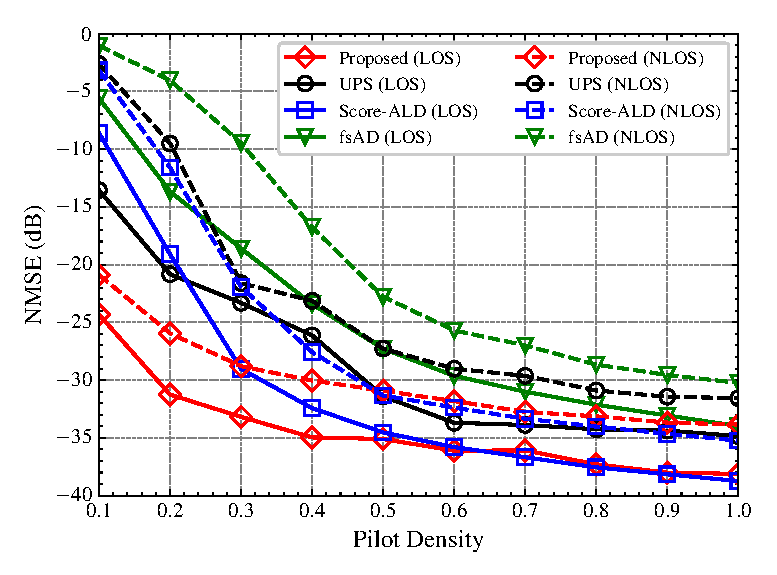
\includegraphics[width=0.48\textwidth]{images/20251014/fig_1.eps}
\caption{Impact of pilot density on the NMSE performance at SNR of 30dB for LOS and NLOS channels.}
\label{fig_sim_1}
\end{figure}

Fig.~\ref{fig_sim_1} illustrates the NMSE performance versus pilot density ($\rho$) at a fixed SNR of 30 dB. The results first highlight the superiority of data-driven generative priors. The fsAD, relying on a hand-crafted sparsity prior, exhibits the most abrupt performance degradation, demonstrating the limitations of a simple structural assumption in the highly uncertain pilot-scarce condition ($\rho<$ 0.5).
While DM-based methods like Score-ALD and UPS are significantly more robust than fsAD, they also suffer from a notable, although less severe, abrupt performance degradation. This degradation indicates that their heuristic likelihood approximations are still insufficient to fully resolve the high uncertainty from limited measurements.
In contrast, the proposed method effectively mitigates this limitation, showing only a gradual performance degradation. This results in a substantial gain of over 10 dB against both Score-ALD and UPS at $\rho$=0.2. This superior pilot efficiency is achieved by incorporating the denoising posterior covariance via Tweedie's formula. This covariance acts as a powerful, data-driven regularizer that effectively constrains the solution space, demonstrating a clear advantage over both conventional CS and other advanced DM-based methods.

\begin{figure}[!t]
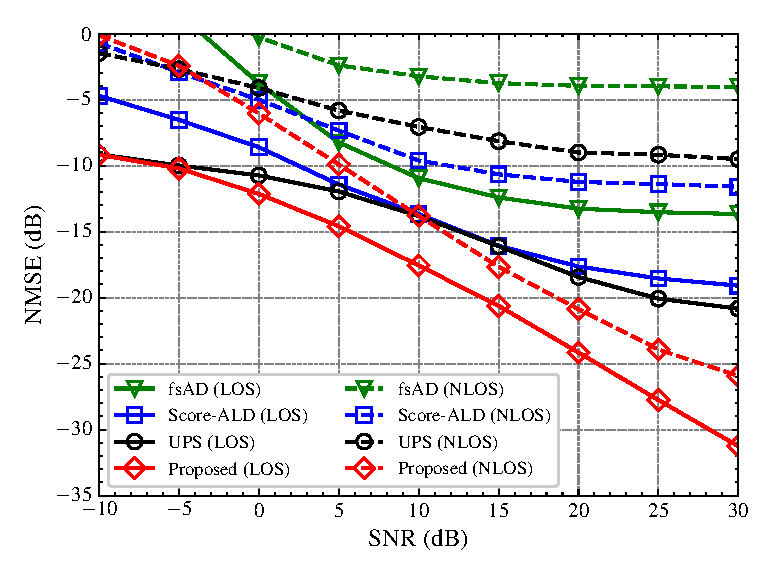
\includegraphics[width=0.48\textwidth]{images/20251014/fig_2.eps}
\caption{Impact of SNR on the NMSE performance with pilot density of 0.2 for LOS and NLOS channels.}
\label{fig_sim_2}
\end{figure}

Fig.~\ref{fig_sim_2} presents the NMSE performance versus SNR at a fixed pilot density of $\rho$=0.2 to evaluate estimation fidelity. The fsAD shows a distinct error floor around -14 dB due to the mismatch between its fixed sparsity assumption and the true channel structure. While all DM-based methods overcome this model mismatch, they exhibit their own error floors except the proposed method. UPS and Score-ALD show floors around -21 dB and -19 dB, respectively, due to algorithmic approximation errors. In sharp contrast, the proposed method exhibits a nearly linear performance improvement as the SNR increases, achieving an NMSE below -30 dB without exhibiting an error floor. Theses results demonstrate that the proposed moment matching-based approach is highly effective. \tblue{By incorporating the denoising posterior covariance, error accumulation can be minimized. This eliminates the approximation-induced error floor that plagues other advanced estimators.} % algorithm 설명에 가까움

Table~\ref{tab:table1} summarizes the computational efficiency of the proposed method. Notably, the proposed method is approximately 65 times faster than Score-ALD.This latency reduction is due to requiring significantly fewer neural function evaluations (NFEs), in contrast to Score-ALD's iterative annealed Langevin dynamics. While it has a slightly higher per-step complexity than UPS, this added computation is targeted. Specifically, the additional operations are dedicated to estimating the denoising posterior covariance using Tweedie's formula, a core component of the moment matching approach. This necessary increase in the complexity of the proposed method is primarily responsible for removing the performance-limiting error floors observed in the baseline methods, as shown in Fig.~\ref{fig_sim_2}. Therefore, the minor computational overhead per step is a highly effective investment, translating directly into state-of-the-art estimation accuracy.

\begin{table}[!t]
\centering
\renewcommand{\arraystretch}{1.1} 
\caption{Computational complexity \\for DM-based channel estimation methods}
\label{tab:table1}
\begin{tabular}{M{0.20\columnwidth}|M{0.21\columnwidth}|M{0.20\columnwidth}|M{0.20\columnwidth}}
\hline
\textbf{Method} & \textbf{FLOPs} & \textbf{NFEs} & \textbf{Latency (s)} \\
\hline
Proposed & \(4.899 \times 10^9\) & 20 & 1.29 \\
\hline
Score-ALD\cite{arvinteMIMOChannelEstimation2023} & \(1.028 \times 10^{12}\) & 6933 & 84.97 \\
\hline
UPS\cite{zhouGenerativeDiffusionModels2025} & \(3.184 \times 10^{10}\) & 130 & 1.27 \\
\hline
\end{tabular}
\end{table}

\section{Conclusions}

In this letter, we proposed a novel channel estimation method for massive MIMO systems. The method effectively addresses estimation accuracy, pilot overhead, and computational complexity. The proposed approach performs accurate and efficient diffusion posterior sampling. It incorporates the denoising posterior covariance based on the moment matching principle and Tweedie's formula. This component proved crucial for overcoming the performance degradation observed in pilot-scarce conditions. From the simulation results, it was demonstrated that the proposed method achieves superior estimation accuracy compared to state-of-the-art baselines. This advantage is particularly pronounced under severe pilot scarcity. Furthermore, it eliminates the error floor present in other advanced estimators at high SNRs. These gains are achieved while maintaining a comparable computational complexity. In future work, the extension of the proposed method to wideband and multi-user scenarios can be explored.
\bibliographystyle{IEEEtran}
% \bibliography{bib/IEEEabrv,bib/references}
\bibliography{bib/references}
\end{document}

